\documentclass{article}
  \usepackage[total={8cm,21cm},top=2cm, left=2cm]{geometry}
  %Paquetes adicionales
  \usepackage{latexsym,amsmath,amssymb,amsfonts}
  \usepackage[latin1]{inputenc}
  \usepackage[T1]{fontenc}
  \usepackage{graphicx}
  \usepackage[spanish]{babel} % Idioma espa�ol
\renewcommand{\baselinestretch}{1.1} % espaciado 1.1
\pagestyle{myheadings}
\markright{...... texto .......} % Encabezados simples
\usepackage{multicol}
\usepackage{xcolor}
\usepackage{pstricks}
\usepackage{marginnote}
\newcommand{\R}{\mathbb{R}}
\newcommand{\Q}{\mathbb{Q}}
\newcommand{\Z}{\mathbb{Z}}
\newcommand{\I}{\mathbb{I}}
\newcommand{\C}{\mathbb{C}}
\newcommand{\E}{\mathbb{E}}
\newcommand{\N}{\mathbb{N}}
\usepackage[shortlabels]{enumitem}
%En el preámbulo
\usepackage{tikz}
%Define un comando para bolas 3D numeradas y de color azul
\newcommand*{\itembolasazules}[1]{% l
\footnotesize\protect\tikz[baseline=-3pt]%
\protect\node[scale=.7, circle, shade,
ball color=blue]{\color{white}\Large\bf#1};}
\usepackage{makeidx}
\makeindex% comentario: para poder visualizar el paquete primero se debe compilar PDF LATEX - makeindez - PDF LATEX
\usepackage{anyfontsize}
\usepackage{fix-cm}
\usepackage{calligra}
\usepackage{mathptmx}
\usepackage{fancyvrb}
\usepackage{esvect}
\usepackage{xargs}
\newcommandx\mpage[4][1=0.45,2=0.45]{%Default=45% ancho página
\begin{minipage}{\textwidth}
\begin{minipage}[b]{#1\textwidth}
#3
\end{minipage} \hfill \begin{minipage}[b]{#2\textwidth}
#4
\end{minipage}
\end{minipage}
}%fin
\newcommand{\limite}[2] { \lim_{ #1 \rightarrow #2}}
\newcommandx\coord[3][1=0, 3=n]{\left(#2_{#1},\ldots,#2_{#3}\right)}
\usepackage[x11names,table]{xcolor}
\usepackage{booktabs}
\usepackage{longtable}
\usepackage{rotating}
\usepackage{epstopdf}
\usepackage{caption}
\usepackage{float}
\usepackage{subfigure}
\begin{document} 

\begin{figure}[h!]
\centering
\subfigure[Converge]{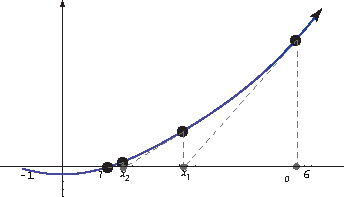
\includegraphics[scale=0.5]{images/newton6}}
\subfigure[Diverge]{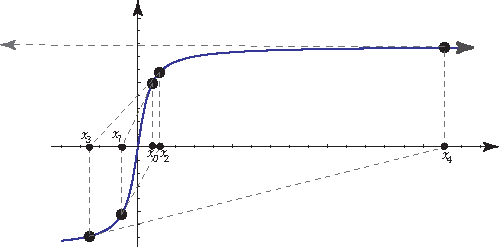
\includegraphics[scale=0.5]{images/newton5}}
\subfigure[Ciclo]{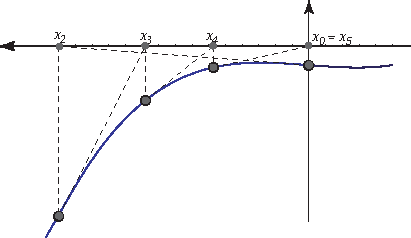
\includegraphics[scale=0.5]{images/newton4}}
\caption{Iteraci�n de Newton}
\end{figure}

\end{document}